\noindent
BALL (Biochemical ALgorithms Library) is an application framework for rapid
software prototyping in the field of Molecular Modeling.  This tutorial shall
help new users to make their first steps with BALL. It is {\em not} a full
documentation. For a full documentation, please refer to the \newterm{Reference
Manual}~\cite{BALL-RM} which can be obtained in HTML, PDF, or postscript format.

There are also several papers and technical reports published on
BALL~\cite{BKL99a,BKL99b,KL99,Koh2001,KL2000,MHLK05,MHLK06}
that give a cursory overview of its design principles and illustrate its use in
Rapid Software Prototyping. If you publish results that were obtained using 
BALL, please cite it as follows:
\begin{enumerate}
  \item[] O. Kohlbacher, H.-P. Lenhof: BALL -- Rapid Software Prototyping
          in Computational Molecular Biology, {\em Bioinformatics} 2000,
          16(9):815--824
\end{enumerate}

\noindent
The latest version of BALL, bug fixes, and updates are available from our 
website

\begin{enumerate}
  \item[] \URL{http://www.ball-project.org}
\end{enumerate}

\noindent 
as well as further documentation, bug reports, and changes.

The next section of this tutorial gives a short overview of the structure and
contents of BALL. Chapter \ref{chapter:getting-started} describes the
installation and related issues. In Chapter \ref{chapter:first-steps}, some
fundamental concepts and classes are explained. After that we will show how to
use more advanced features of BALL. We will have a general overview of BALL 
 (Chapters \ref{chapter:foundation-classes} and  \ref{chapter:kernel}) 
and the usage of the visualization parts of BALL (Chapter \ref{chapter:view-programming}). 
Chapter \ref{chapter:python} will show you
the mechanisms and the usage of BALL's Python bindings.  Finally, Chapter
\ref{chapter:faq} tries to answer some of the most frequently asked questions.

\section{Overview}
\index{BALL!overview}

The basis of all BALL classes is an extensive set of \newterm{foundation
classes}.  They provide generic implementations of advanced data structures
(\eg, trees, hash associative containers, hash grids, \etc), mathematical
objects (\eg, matrices, vectors, geometric objects), implementations of
\Index{design patterns}, object \Index{persistence}, and access to the
operating system (\eg, networking support, file handling). An overview of the
overall structure of BALL is given in Fig. \ref{fig:BALL_structure}.

The BALL \newterm{kernel} contains the molecular data structures for the
representation of atoms, bonds, molecules, proteins, \etc  The kernel classes
are implemented with the foundation classes and are carefully designed to
provide maximum extensibility and flexibility.
\begin{figure}[tb]
  \centering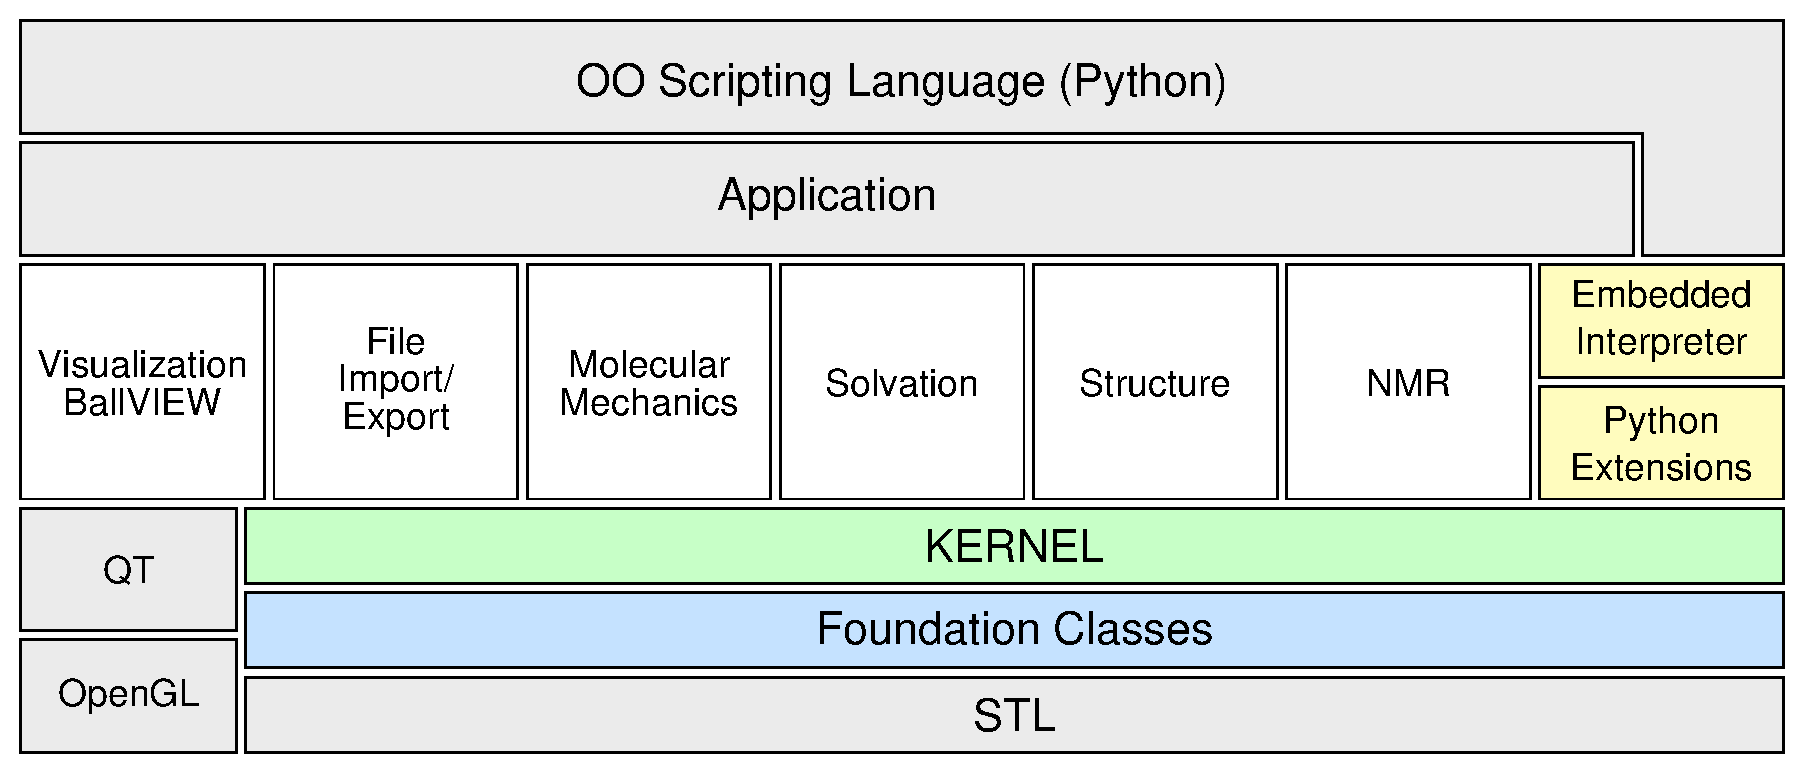
\includegraphics[width=\textwidth]{BALL_structure.eps}
  \caption{Overview of the structure of BALL}
  \label{fig:BALL_structure}
\end{figure}

The third layer of classes (on top of the foundation classes and the kernel)
provides the functionality required for applications. We call them
\newterm{basic components}. Each of these basic components is independent of
the other components.  We have implemented five basic components that cover
\Index{Molecular Mechanics}, file import/export, advanced \Index{solvation
methods}, structure analysis/comparison and \Index{visualization}. These
areas were selected, because our main interest stems from the field of protein
docking. The Molecular Mechanics component does not only provide standard
force fields (AMBER~\cite{AMBER95}, CHARMM~\cite{BBO+83},
MMFF~\cite{MMFF94a,MMFF94b,MMFF94c,MMFF94d,MMFF94e}), but also a generic
\Index{force field}.  This generic force field is a base class for all force
fields. It implements fundamental methods to manage parameter files, parameter
assignment, and atom type assignment, and defines a common interface for all
force fields. Thus, large portions of code may be reused for the
implementation of new force fields.  The file import/export component
implements general methods for efficient file handling, but also methods to
read and write the most common file formats used for molecular structures
(\eg, PDB, MOL2, HIN). The solvation component provides methods for calculating
solvation effects. The first method that accounts for solvation is the atomic
contact energy by Zhang {\it et al.}~\cite{ZVC+97}. The second approach that
we implemented is a numerical solver for the \Index{Poisson-Boltzmann} equation.  The
structure component contains algorithms to search for common structural motifs
in proteins, to map molecules onto each other, and to calculate solvent
accessible and solvent excluded surfaces of molecules. For the visualization
of the results, we designed \Index{VIEW}, a class hierarchy that
visualizes BALL kernel objects with standard representations (ball and stick,
van der Waals, ribbons, surfaces, \etc). The visualization was implemented
using OpenGL~\cite{OpenGL} and Qt~\cite{QT}. Hence, it is highly portable and 
enables the user to produce state-of-the-art graphical user interfaces with a
minimum effort.

The fourth layer in BALL consists of Python bindings. Python~\cite{Python} is
an object-oriented scripting language that is easy to learn and very readable.
BALL provides Python bindings for most of its classes, which allow the use of
the BALL \CPP classes from Python. This approach drastically reduces the
turn-around times (no compiling and linking phase is required) and adds
scripting capabilities to BALL without introducing a new and exotic scripting
language. The Python bindings use the same class names as the BALL classes,
therefore after the initial rapid development of a methodology, the existing
Python code can be easily ported back to \CPP for production purposes.
Chapter \ref{chapter:python} gives a short introduction to this feature.
